\documentclass[11pt,a4paper]{article}
\usepackage[margin=2.3cm]{geometry}
\usepackage{amsmath,amssymb}
\usepackage{graphicx}
\usepackage{booktabs}
\usepackage{siunitx}
\usepackage{xcolor}
\usepackage[colorlinks=true,linkcolor=blue!50!black,citecolor=blue!50!black,urlcolor=blue!50!black]{hyperref}
\usepackage{microtype}
\usepackage{caption}
\captionsetup{font=small,labelfont=bf,width=0.95\textwidth}
\graphicspath{{figs/}}
\newcommand{\nD}{20000000}
\newcommand{\nN}{20000000}
\newcommand{\nP}{20000000}
\newcommand{\nDM}{20}
\newcommand{\meanHi}{0.9944}
\newcommand{\meanHiErr}{0.0003}
\newcommand{\minLo}{9.2}
\newcommand{\minHi}{9.3}
\newcommand{\minRat}{0.9889}
\newcommand{\minErr}{0.0016}
\newcommand{\maxLo}{8.6}
\newcommand{\maxHi}{8.7}
\newcommand{\maxRat}{1.0173}
\newcommand{\maxErr}{0.0023}
\newcommand{\totalRatio}{1.0321}
\newcommand{\noFluxTotal}{0.9919}
\newcommand{\meanFlux}{1.0405}
\newcommand{\ratA}{1.7757}
\newcommand{\ratErrA}{0.0047}
\newcommand{\ratNFA}{1.6225}
\newcommand{\yOnA}{7.78}
\newcommand{\yOffA}{4.38}
\newcommand{\ratB}{1.0879}
\newcommand{\ratErrB}{0.0020}
\newcommand{\ratNFB}{1.0149}
\newcommand{\yOnB}{12.01}
\newcommand{\yOffB}{11.04}
\newcommand{\ratC}{0.9992}
\newcommand{\ratErrC}{0.0010}
\newcommand{\ratNFC}{0.9486}
\newcommand{\yOnC}{37.79}
\newcommand{\yOffC}{37.82}
\newcommand{\ratD}{0.9902}
\newcommand{\ratErrD}{0.0007}
\newcommand{\ratNFD}{0.9518}
\newcommand{\yOnD}{73.54}
\newcommand{\yOffD}{74.27}
\newcommand{\ratE}{0.9929}
\newcommand{\ratErrE}{0.0006}
\newcommand{\ratNFE}{0.9611}
\newcommand{\yOnE}{103.11}
\newcommand{\yOffE}{103.84}
\newcommand{\ratF}{0.9961}
\newcommand{\ratErrF}{0.0005}
\newcommand{\ratNFF}{0.9679}
\newcommand{\yOnF}{156.09}
\newcommand{\yOffF}{156.70}
\newcommand{\photonsInRange}{1.439}
\newcommand{\photonsAboveTh}{0.768}
\newcommand{\tipLoss}{1.24}
\newcommand{\Satiii}{0.968}
\newcommand{\Sati}{0.910}
\newcommand{\Satxxx}{0.769}
\newcommand{\Satx}{0.582}
\newcommand{\Satc}{0.362}
\newcommand{\Sata}{0.160}
\newcommand{\fracBelow}{2.55}
\newcommand{\yieldBelow}{10.21}
\newcommand{\fracBelowEight}{1.41}
\newcommand{\fracBelowSeven}{0.33}
\newcommand{\cntA}{13282}
\newcommand{\cntB}{52273}
\newcommand{\cntC}{216927}
\newcommand{\cntD}{227595}
\newcommand{\psAb}{99}
\newcommand{\fpsAb}{4.4}
\newcommand{\msAb}{0.915}
\newcommand{\nspAb}{19489923}
\newcommand{\psBe}{229}
\newcommand{\fpsBe}{26.2}
\newcommand{\msBe}{0.840}
\newcommand{\nspBe}{510077}
\newcommand{\psEi}{278}
\newcommand{\fpsEi}{36.2}
\newcommand{\msEi}{0.807}
\newcommand{\nspEi}{282482}
\newcommand{\psSe}{400}
\newcommand{\fpsSe}{67.6}
\newcommand{\msSe}{0.706}
\newcommand{\nspSe}{65555}
\newcommand{\yieldD}{400.52}
\newcommand{\sigD}{0.2783}
\newcommand{\yieldN}{388.06}
\newcommand{\sigN}{0.2696}
\newcommand{\yieldP}{332.82}
\newcommand{\sigP}{0.2677}

\sisetup{separate-uncertainty=true}

\newcommand{\Eg}{E_\gamma}
\newcommand{\jpsi}{J/\psi}
\newcommand{\nb}{\,\mathrm{nb}}
\newcommand{\GeV}{\,\mathrm{GeV}}
\newcommand{\ps}{p_s}

\title{Fermi motion in untagged $\jpsi$ photoproduction on the deuteron\\
\large Bremsstrahlung photon beam from the 5\,cm target, spectator model of the deuteron,\\
and the yield ratio to a free neutron at rest}
\author{V.~Kubarovsky\\ \small Thomas Jefferson National Accelerator Facility\\
\small generator: \texttt{exclurad\_py}, branch \texttt{jpsi-fermi}, module \texttt{generator/photo.py}}
\date{26 September 2026}

\begin{document}
\pagestyle{plain}
\maketitle

\begin{abstract}
\noindent
A 10.6\,GeV electron beam radiates in the 5\,cm liquid-deuterium cell of CLAS12 and the bremsstrahlung
photons produce $\jpsi$ mesons on the neutrons of the deuteron, $\gamma n\to\jpsi\,n$.  We describe the
photon spectrum used, including the correct behaviour at the endpoint $\Eg\to E_0$ where the
complete-screening formula fails, the spectator model of the deuteron with the AV18 momentum
distribution, and the Monte Carlo that combines them with the $\jpsi$ cross section of the
\texttt{roberts2026} parametrisation.  With $\nDM$ million events per sample the ratio of the $\jpsi$
yield per neutron on the deuteron to the yield on a free neutron at rest is measured to \num{0.2}\,\%
per 100\,MeV bin of photon energy.  Above $\Eg=8.6\GeV$ the ratio stays between $\minRat$ and
$\maxRat$, with a mean of $\meanHi\pm\meanHiErr$: Fermi motion changes the yield per neutron by less
than 1\,\%.  Two effects of comparable size and opposite sign make up this
number: the binding of the struck neutron lowers the available $\gamma n$ energy and reduces the yield
by about 4\,\%, and the M\o{}ller flux factor of the moving neutron, correlated with the steeply
rising cross section, raises it by about the same amount.  Fermi motion is therefore negligible for the
yield above 8.6\,GeV, but the shape of the ratio near the free threshold at 8.20\,GeV and the yield
below it, $\fracBelow\,\%$ of the total, are entirely due to it.  It also dominates the resolution of
every quantity reconstructed with the target assumed at rest: the photon energy obtained from the
$\jpsi$ alone is smeared by $\erRH$\,MeV rms and shifted by up to $\erBB$\,MeV near threshold.  The
conclusion (Section~\ref{sec:need}) is that the Monte Carlo has to include Fermi motion for any
analysis on deuterium, although the generated yield per neutron above 8.6\,GeV does not require it.
\end{abstract}

\tableofcontents

\section{Purpose and set-up}

The question asked was simple: how much does the Fermi motion of the neutron in the deuteron change the
$\jpsi$ photoproduction yield in the CLAS12 configuration, where the photon beam is the untagged
bremsstrahlung of the 10.6\,GeV electron beam in the target itself?  The scattered electron is not
observed; it stays in the beam line.  The observable is the $\jpsi\to e^+e^-$ yield as a function of
the photon energy reconstructed from the final state, and its $t$ distribution.

The generator therefore has three ingredients, described in the next three sections:
\begin{enumerate}
\item the photon spectrum $dN_\gamma/d\Eg$ per incident electron, from thin-target bremsstrahlung in
      the cell, with the endpoint treated correctly (Section~\ref{sec:brems});
\item the deuteron, in the plane-wave spectator model with the AV18 momentum distribution
      (Section~\ref{sec:deuteron});
\item the elementary cross section $\sigma(\gamma N\to\jpsi N)$ and its $t$ dependence
      (Section~\ref{sec:model}).
\end{enumerate}
Section~\ref{sec:generator} gives the algorithm and its validation, Section~\ref{sec:results} the
results of the high-statistics samples, and Section~\ref{sec:discussion} the interpretation and the
limits of the model.  All samples were produced with \texttt{exclurad\_py} on the \texttt{jpsi-fermi}
branch; the cards and commands are in Appendix~\ref{app:cards}.

Three samples are compared throughout, all with the same photon spectrum and the same elementary cross
section:
\begin{center}
\begin{tabular}{lp{8.5cm}r}
\toprule
sample & target & events \\
\midrule
\textbf{deuteron} & neutron of the deuteron, AV18 Fermi motion, spectator proton written out & $\nD$ \\
\textbf{neutron}  & free neutron at rest & $\nN$ \\
\textbf{proton}   & free proton at rest (LH$_2$ radiator thickness), for cross-checks & $\nP$ \\
\bottomrule
\end{tabular}
\end{center}
The \emph{deuteron}/\emph{neutron} ratio, yield per neutron, isolates the effect of Fermi motion and
binding; the photon flux and the cross section cancel in it bin by bin.

\section{The photon beam: bremsstrahlung in the target}
\label{sec:brems}

\subsection{Thin-target spectrum}

The beam electron of energy $E_0=10.6\GeV$ traverses the liquid target and radiates.  The 5\,cm cell is
$L/X_0 = 5/769.1 = 6.5\times10^{-3}$ radiation lengths of LD$_2$ ($5.6\times10^{-3}$ for LH$_2$,
$X_0=890.4$\,cm), so the thin-target formula applies: the photon spectrum is linear in the thickness
and the energy loss of the electron before it radiates is neglected (it is at most 1.7\,MeV over the
full cell, see Section~\ref{sec:endpoint}).  We use the complete-screening form of Tsai,
\begin{equation}
\frac{dN_\gamma}{d\Eg}\,=\,\frac{X}{X_0}\;\frac{1}{\Eg}\Bigl[\tfrac43\,(1-y)+y^2\Bigr]\,S(\Eg),
\qquad y=\frac{\Eg}{E_0},
\label{eq:tsai}
\end{equation}
where $X$ is the thickness of material the electron has crossed before the production vertex and
$S(\Eg)$ is the endpoint factor of Section~\ref{sec:endpoint}, equal to one except in the last
$\sim$300\,MeV.  The definition of $X_0$ absorbs the atomic screening logarithms and the contribution
of the atomic electron, which for hydrogen and deuterium is as large as that of the nucleus.

The photon flux grows linearly along the cell, so the production vertices are distributed with a
density proportional to the upstream thickness, $dP/dz\propto z-z_{\rm in}$; the generator draws
$z = z_{\rm in} + L\sqrt{u}$ with $u$ uniform.  Integrated over the cell, the yield per incident
electron and per target nucleon is that of the average thickness, $X=L/2$, and this is the factor used
in the event weight,
\begin{equation}
\frac{X}{X_0}=\frac{L}{2X_0}=3.25\times10^{-3}\ \text{(LD$_2$)},\qquad 2.81\times10^{-3}\ \text{(LH$_2$)}.
\end{equation}
With these numbers the LD$_2$ cell delivers $\photonsInRange\times10^{-3}$ photons per electron
between 6.5 and 10.6\,GeV, and $\photonsAboveTh\times10^{-3}$ above the free-neutron threshold of
8.20\,GeV (Figure~\ref{fig:flux}, left).

\subsection{The endpoint}
\label{sec:endpoint}

Formula~(\ref{eq:tsai}) without $S$ is finite at $\Eg=E_0$: the bracket tends to one and the spectrum
to $1/E_0$.  This is an artefact of the complete-screening approximation, which assumes that the
minimum momentum transfer to the atom,
\begin{equation}
q_{\min}=\frac{m_e^2\,\Eg}{2E\,E'},\qquad E=E_0,\ E'=E_0-\Eg,
\end{equation}
is small compared with the inverse screening radius $1/a_s$ of the atomic electron cloud.  As
$E'\to0$ the momentum transfer grows without bound, screening switches off, and the cross section is
governed by the unscreened logarithm $\ln(2EE'/m_e\Eg)$, which falls through zero when $E'$ becomes of
the order of $m_e$.  \textbf{The spectrum therefore does go to zero at the endpoint}, over the last
fraction of an MeV, after bending down over the last few tens of MeV.

We use the analytic intermediate-screening spectrum of Schiff (Koch and Motz formula 3BS(b)), which
interpolates between complete and no screening with the momentum transfer of each photon energy.  With
$r=E'/E$ and, in units of $m_e$,
\begin{equation}
b=\frac{2EE'}{a_s\,\Eg},\qquad
\frac{1}{M(0)}=\Bigl(\frac{\Eg}{2EE'}\Bigr)^2+\frac{1}{a_s^2},
\end{equation}
Schiff's spectrum is
\begin{align}
\frac{d\sigma}{d\Eg}\,\propto\,\frac{1}{\Eg}\Bigl\{&
\Bigl[1+r^2-\tfrac23 r\Bigr]\Bigl[\ln M(0)+1-\tfrac{2}{b}\arctan b\Bigr]\nonumber\\
&+\,r\Bigl[\tfrac{2}{b^2}\ln(1+b^2)+\tfrac{4(2-b^2)}{3b^3}\arctan b-\tfrac{8}{3b^2}+\tfrac29\Bigr]\Bigr\}.
\label{eq:schiff}
\end{align}
Its complete-screening limit $b\to\infty$ is $\frac1{\Eg}\{[1+r^2-\frac23 r](2\ln a_s+1)+\frac29 r\}$,
and $1+r^2-\frac23 r=\frac43(1-y)+y^2$ is exactly the Tsai bracket.  The endpoint factor is the ratio
\begin{equation}
S(\Eg)=\frac{\text{Eq.~(\ref{eq:schiff})}}{\text{its complete-screening limit}},
\end{equation}
cut at zero where Schiff's bracket turns negative, and it multiplies the Tsai shape in
Eq.~(\ref{eq:tsai}).  Applying the ratio rather than Eq.~(\ref{eq:schiff}) itself keeps the
normalisation of $X_0$, which contains the electron contribution and the Coulomb-free $Z=1$
logarithms, and changes only the shape where the physics changes.

The screening radius is the one parameter.  Schiff's Thomas--Fermi value $a_s=111\,Z^{-1/3}$ (in
Compton wavelengths) describes many-electron atoms; hydrogen and deuterium have a single $1s$ electron
and the physical screening length is the Bohr radius, $a_0=\lambda_C/\alpha=137$ Compton wavelengths.
We use 137; Figure~\ref{fig:flux} (right) shows that the difference from 111 is confined to the last
few MeV.  The resulting factor is
\begin{center}
\begin{tabular}{lcccccc}
\toprule
$E_0-\Eg$ [MeV] & 300 & 100 & 30 & 10 & 3 & 1 \\
$S(\Eg)$ & \Satiii & \Sati & \Satxxx & \Satx & \Satc & \Sata \\
\bottomrule
\end{tabular}
\end{center}
and $S=0$ for $E_0-\Eg<0.42$\,MeV.  The endpoint correction removes $\tipLoss\,\%$ of the photons
between 6.5 and 10.6\,GeV.  Its effect on the $\jpsi$ yield is proportionally larger than on the photon
count, because the cross section is largest at the highest photon energies, but it is still a
sub-percent effect on the total; what it does change is the last 100\,MeV of the $\Eg$ spectrum, which is
what a measurement near the endpoint sees.

Three effects that we do not include act on the same scale.  The electron loses up to 1.7\,MeV by
ionisation before it radiates ($dE/dx\simeq0.35$\,MeV/cm in LD$_2$), the CEBAF beam has an energy
spread of order $10^{-4}$, i.e.\ 1\,MeV, and the bremsstrahlung on the atomic electron has its own
endpoint $1.5\,m_e$ below $E_0$.  Each smears or shifts the tip by about 1\,MeV; none matters for the
$\jpsi$ yield.  In the last 5\,MeV the formula is also outside its domain, $E'\gg m_e$; that region
holds less than $10^{-4}$ of the photons above 6.5\,GeV.

\begin{figure}[htbp]
\centering
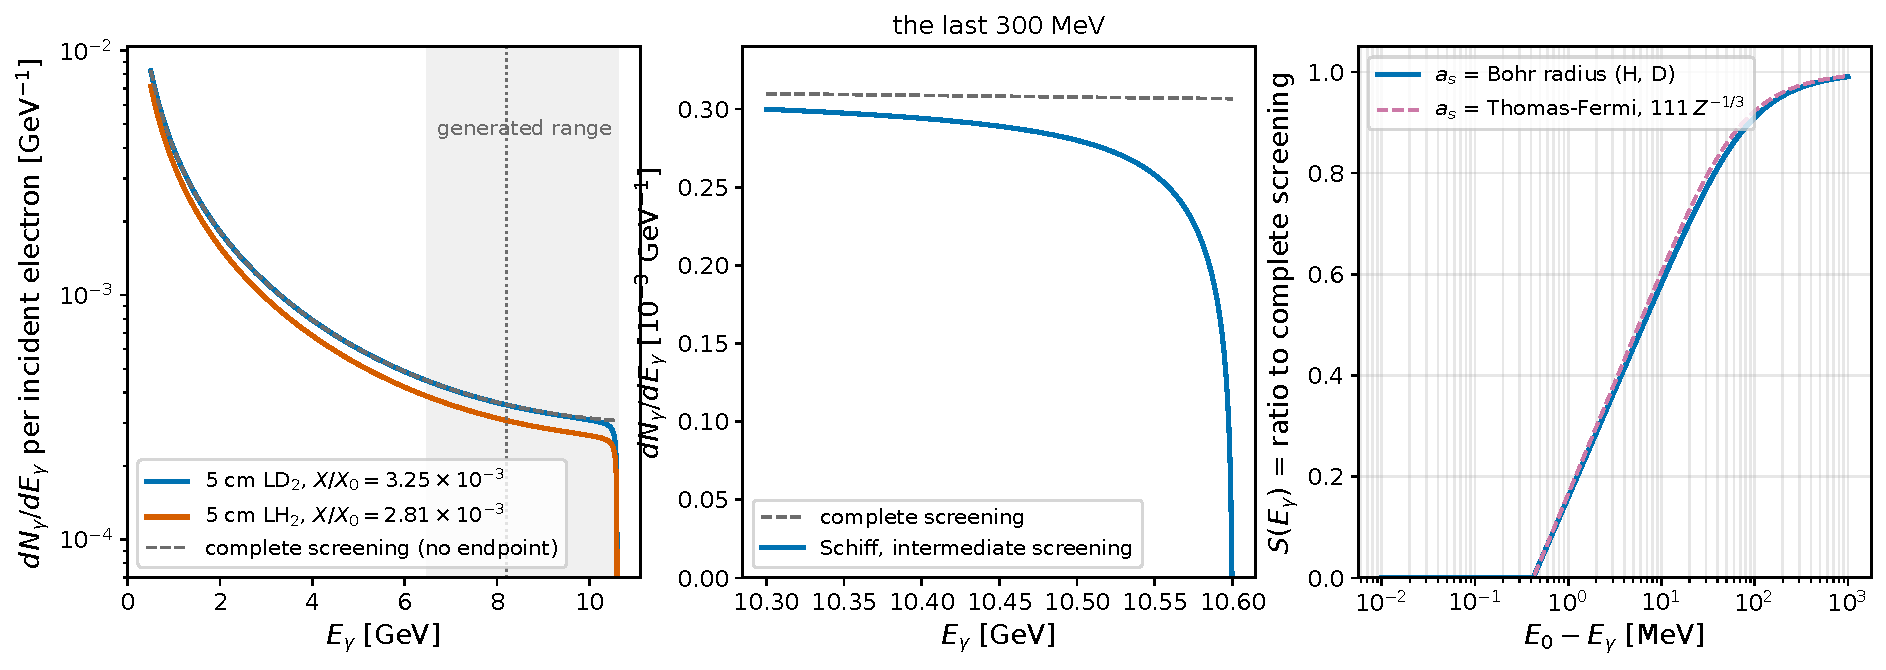
\includegraphics[width=\textwidth]{fig_flux}
\caption{The photon beam.  Left: photons per incident electron and per GeV from the 5\,cm cell
(average upstream thickness $L/2$), for LD$_2$ and LH$_2$; the dashed curve is the complete-screening
formula without the endpoint factor; the shaded band is the generated range 6.5--10.6\,GeV and the
dotted line the free-neutron threshold.  Middle: the last 300\,MeV, where the Schiff intermediate
screening spectrum bends down and reaches zero at the endpoint while the complete-screening formula
stays finite.  Right: the endpoint factor $S(\Eg)$ against the distance to the endpoint, for the Bohr
radius used here and for Schiff's Thomas--Fermi radius.}
\label{fig:flux}
\end{figure}

\section{The deuteron: spectator model}
\label{sec:deuteron}

The deuteron is at rest in the laboratory.  In the plane-wave spectator picture the photon interacts
with one nucleon while the other is a spectator that leaves with the momentum it had in the nucleus.
The spectator is on its mass shell, the struck nucleon carries the rest of the deuteron four-momentum
and is off shell:
\begin{equation}
p_s=(E_s,\vec\ps),\quad E_s=\sqrt{M_p^2+\ps^2};\qquad
p_N=(M_D-E_s,\,-\vec\ps),\qquad m^{*2}=p_N^2<M_n^2 .
\end{equation}
The spectator momentum is drawn from the AV18 deuteron momentum distribution $n(\ps)$ ($S$ and $D$
waves, normalised to one, tabulated up to $\ps=0.70$\,GeV/$c$), isotropic in the laboratory.  The
photon--neutron invariant mass is built from the actual four-vectors,
\begin{equation}
s=(k+p_N)^2=m^{*2}+2\Eg\,(E_N-p_{N,z}),
\end{equation}
so a neutron running toward the photon ($p_{N,z}<0$) raises $s$ and one running away lowers it.  The
free-neutron threshold $\Eg^{\rm th}=[(M_n+M_{\jpsi})^2-M_n^2]/2M_n=8.20\GeV$ is no longer a
threshold: the reaction $\gamma d\to\jpsi\,n\,p$ is open from $[(M_{\jpsi}+M_n+M_p)^2-M_D^2]/2M_D
=5.66\GeV$, and photons between 5.66 and 8.20\,GeV produce $\jpsi$ on the high-momentum tail of
$n(\ps)$.  The generated range starts at 6.5\,GeV; below it the yield is negligible
(Section~\ref{sec:below}).

Two conventions of the earlier electroproduction study are kept.  The cross section is evaluated at the
free-nucleon mass, as a function of the invariants $s$ and $t$ of the event, and $m^*$ enters only
where the event is built, i.e.\ in the kinematics of the final state.  And a draw with
$m^*<0.10\GeV$ is rejected: there the struck nucleon becomes light-like and the plane-wave picture
has no meaning.  The floor was chosen for this study from the table of allowed configurations
(Table~\ref{tab:floor}): at 7.0\,GeV, where only 0.9\,\% of the AV18 configurations can produce a
$\jpsi$ at all, the floor at 0.30\,GeV used for $\pi^0$ would remove 3\,\% of them, the floor at
0.10\,GeV removes 0.1\,\%.

\begin{table}[htbp]
\centering
\caption{Kinematics of the struck neutron in the deuteron for a photon along $+z$ (AV18, 200\,000
configurations, unweighted by the cross section): fraction of configurations above the $\jpsi$
threshold, their mean spectator momentum, the fraction with $\ps>300$\,MeV/$c$, and the fraction of
the allowed configurations removed by a floor on $m^*$.}
\label{tab:floor}
\begin{tabular}{ccccccc}
\toprule
$\Eg$ [GeV] & allowed & $\langle\ps\rangle$ [MeV/$c$] & $\ps>300$ & floor 0.30 & 0.20 & 0.10 \\
\midrule
7.0  & 0.88\,\% & 373 & 60.8\,\% & 2.9\,\%  & 0.7\,\%  & 0.11\,\% \\
7.5  & 4.44\,\% & 224 & 18.3\,\% & 0.7\,\%  & 0.2\,\%  & 0.04\,\% \\
8.0  & 24.6\,\% & 117 & 4.4\,\%  & 0.17\,\% & 0.06\,\% & 0.01\,\% \\
8.2  & 44.3\,\% & 91  & 2.6\,\%  & 0.10\,\% & 0.03\,\% & 0.01\,\% \\
10.0 & 97.3\,\% & 86  & 1.9\,\%  & 0.06\,\% & 0.02\,\% & 0.00\,\% \\
\bottomrule
\end{tabular}
\end{table}

\subsection{The event weight and the flux factor}
\label{sec:flux}

Per incident electron and per target neutron, the number of $\jpsi$ events is
\begin{equation}
dN=\frac{dN_\gamma}{d\Eg}\,d\Eg\;\times\;n(\ps)\,d^3\ps\;\times\;
\frac{k\cdot p_N}{\Eg\,E_N}\;\sigma_{\gamma n}(s)\,,
\qquad \frac{k\cdot p_N}{\Eg\,E_N}=1-\beta_{N,z},
\label{eq:weight}
\end{equation}
where the last factor is the M\o{}ller flux factor of the moving target: the rate of a massless
projectile on a target with velocity $\vec\beta_N$ is $\sigma$ times the relative velocity
$1-\beta_{N,z}$, not $\sigma$ alone.  For a nucleon at rest it is one, and averaged over the isotropic
$n(\ps)$ it is also one.  It is nevertheless not a detail here.  A neutron running toward the photon
has both a larger flux factor and a larger $s$, hence a larger cross section; the two are positively
correlated and the average of the product exceeds the product of the averages.  Because
$\sigma_{\gamma n}(s)$ rises steeply above threshold (Section~\ref{sec:model}), this correlation is
worth about $+4\,\%$ on the deuteron yield at 10\,GeV and more near threshold.  It was absent from the
first version of the generator, and its absence produced a spurious 4\,\% deficit of the deuteron
yield; the samples in this report include it, and Section~\ref{sec:ratio} shows the ratio with and
without it.  The same factor is missing in the electroproduction branch of the generator
(\texttt{generator/fermi.py} working in the struck-nucleon rest frame), where its numerical effect is
much smaller because the $\pi^0$ and $\eta$ cross sections vary slowly with $W$; it should be added
there for consistency.

\section{The elementary cross section}
\label{sec:model}

The hadronic side is the electroproduction model \texttt{jpsi.roberts2026} at $Q^2=0$, relabelled for
a neutron target as \texttt{jpsin.roberts2026} with $\sigma_n=\sigma_p$.  Nothing new is assumed on
this side: in the Hand convention the transverse cross section at $Q^2=0$ \emph{is} the real-photon
cross section, so the generator uses the model's $\sigma_T(W,Q^2\!=\!0,t)$ as $d\sigma/dt$.  The
parametrisation is
\begin{equation}
\sigma_{\rm tot}(W)=A\,(W-W_{\rm th})^{\alpha}\,e^{-B\,(W-W_{\rm th})},\qquad
\frac{d\sigma}{dt}=\sigma_{\rm tot}(W)\;\frac{b\,e^{b\,t'}}{1-e^{-b\,|t'|_{\max}}},\quad t'=t-t_{\min},
\end{equation}
with $A=1.018\nb$, $\alpha=0.707$, $B=-0.928\GeV^{-1}$, $b=1.67\GeV^{-2}$ and $W_{\rm th}=M_N+M_{\jpsi}
=4.036\GeV$.  Between the free threshold and 10.6\,GeV, $W-W_{\rm th}$ runs from 0 to 0.52\,GeV and
$\sigma_{\rm tot}$ from 0 to $1.05\nb$ (Figure~\ref{fig:model}); the logarithmic derivative
$d\ln\sigma/dW=\alpha/(W-W_{\rm th})-B$ is 2.7\,GeV$^{-1}$ at 10\,GeV and diverges at threshold, which
is what makes the deuteron yield sensitive to shifts of $s$ of a few $10^{-2}$\,GeV$^2$.  The $t$ range
generated is $-6\le t\le-0.001\GeV^2$, cut to the physical range at each $W$; $|t|_{\min}$ is 1.8,
0.62 and 0.36\,GeV$^2$ at 8.5, 9.5 and 10.5\,GeV.

Figure~\ref{fig:model} compares the parametrisation with the CLAS12 measurement on the proton
\cite{clas12jpsi} (Tables~V and VI of its Appendix~A).  The total cross section is described within
the errors from threshold to 9.6\,GeV; above 9.7\,GeV the data lie 20--30\,\% above the curve, one to
two standard deviations per point.  The $t$ dependence of the data is compatible with the single
exponential in $t'$ at $|t|\lesssim2\GeV^2$; the points beyond, at 3--4\,GeV$^2$, sit above the
exponential by a factor two to three.  Neither deviation matters for the Fermi-motion ratio of
Section~\ref{sec:ratio}, which depends on the slope of $\sigma(W)$ near threshold and on nothing
else; it would matter for absolute yields, and a refit of $A$, $\alpha$, $B$ and $b$ to these data is
the natural next step.

\begin{figure}[htbp]
\centering
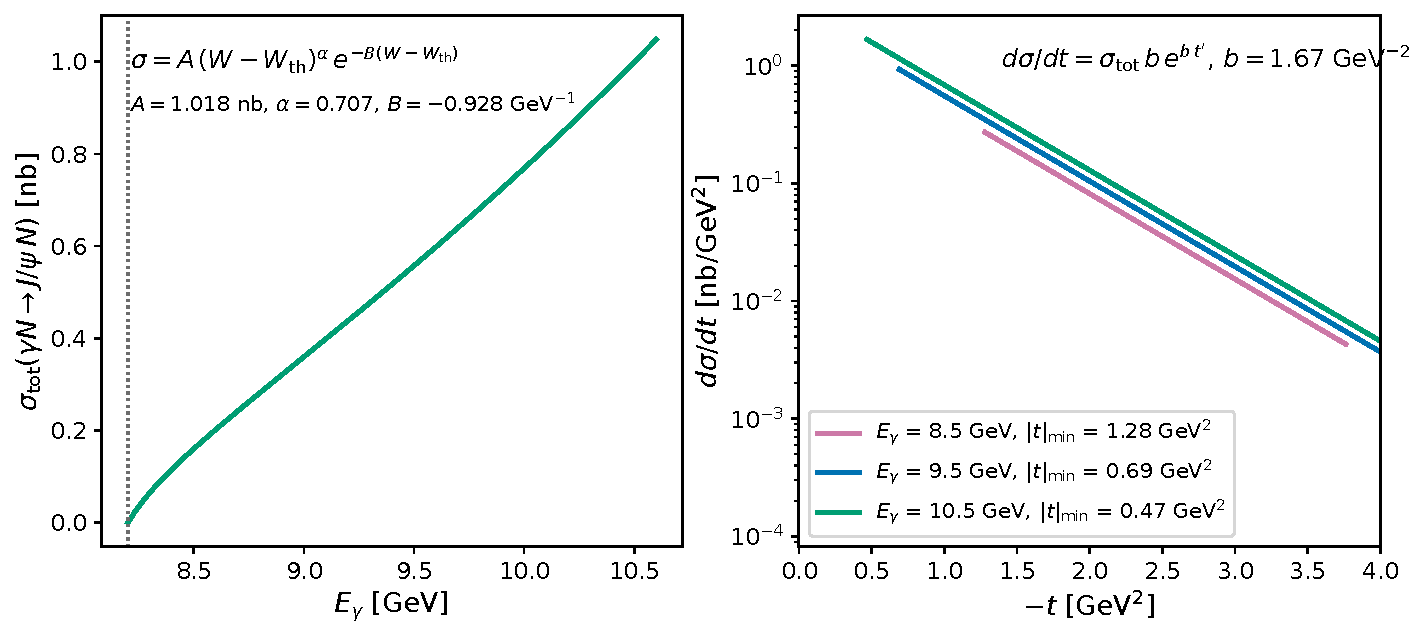
\includegraphics[width=0.95\textwidth]{fig_model}
\caption{The elementary cross section used, compared with the CLAS12 measurement on the proton
(Chatagnon et al.\ 2026, Appendix~A tables).  Left: $\sigma_{\rm tot}(\gamma p\to\jpsi\,p)$ of the
\texttt{roberts2026} parametrisation against the photon energy on a nucleon at rest, with the CLAS12
total cross section in ten energy bins; the inner bar is the statistical error, the outer one
statistical and systematic added in quadrature, the horizontal bar the rms of the photon energy in
the bin.  Right: $d\sigma/dt$ of the model at the mean photon energy of the three CLAS12 energy bins,
with the CLAS12 differential cross sections of those bins (errors as on the left, horizontal bars the
rms of $-t$ in the bin).}
\label{fig:model}
\end{figure}

\section{The generator and its validation}
\label{sec:generator}

\subsection{Algorithm}

Each trial proceeds as follows.
\begin{enumerate}
\item $\Eg$ is drawn from the spectrum~(\ref{eq:tsai}) in $[k_{\min},k_{\max}]$ by a tabulated inverse
      cumulative (20\,001 points), including the endpoint factor.
\item The target nucleon is set at rest, or, on the deuteron, $\vec\ps$ is drawn from AV18, the struck
      four-vector and $m^*$ are formed, and the trial is discarded if $m^*<0.10\GeV$ (0.01\,\% of the
      draws).
\item $s=(k+p_N)^2$ is computed; if it is below $(M_{\jpsi}+M_N)^2$ the trial is counted as below
      threshold and discarded.
\item The trial is accepted with probability $\sigma_{\rm tot}(s)\,(1-\beta_{N,z})/w_{\max}$.
      $\sigma_{\rm tot}(s)$, the $t$ integral of $d\sigma/dt$ over the card's range, is tabulated once
      on an 800-point grid in $s$.  The majorant $w_{\max}$ is the maximum of
      $\sigma_{\rm tot}(s)\,(1-\beta_{N,z})$ along the head-on line, a neutron running toward the
      photon with $\ps$ up to the AV18 ceiling at $k_{\max}$: for a given $|\ps|$ both $s$ and the
      flux factor are largest there, so this is a strict bound and no event is under-weighted (the
      generator counts overweights; there were none).  The price is efficiency: $w_{\max}/\langle
      \sigma\rangle\simeq36$ on the deuteron and 4 on a free nucleon.
\item $t$ is drawn from the exact inverse cumulative of $d\sigma/dt$ at the event's $s$ (401 points),
      $\phi$ uniformly.
\item The $\jpsi$ and the recoil neutron are built in the $\gamma N$ centre of mass and boosted to the
      laboratory with the actual photon and nucleon four-vectors, so on the deuteron
      $k+p_D=p_{\jpsi}+p_{n'}+p_s$ exactly.  The $\jpsi$ is decayed to $e^+e^-$ isotropically.  The
      vertex is drawn along the cell as in Section~\ref{sec:brems}.
\end{enumerate}
The events are written in LUND format with the photon as the beam (pid 22, energy $\Eg$ in the
header), the target pid 2112 or 1000010020, the $\jpsi$ as a status-0 parent with its daughters, the
recoil and, on the deuteron, the spectator proton.  The run's \texttt{config.json} records the photon
count per electron in the generated range, the flux-weighted $\langle\sigma\rangle$, and the yield per
incident electron per target nucleon, $Y=\int d\Eg\,(dN_\gamma/d\Eg)\,\langle(1-\beta_z)\sigma\rangle$.

\subsection{Validation}

\begin{itemize}
\item \textbf{Four-momentum conservation.}  $|k+p_{\rm target}-\sum p_{\rm final}|<5.5\times10^{-9}\GeV$
      for every event of the 200\,000-event test samples, i.e.\ the ten significant digits of the LUND
      file; the spectator is on shell to $3\times10^{-16}$.
\item \textbf{Photon spectrum.}  On the free proton the generated $\Eg$ distribution against the
      analytic $dN_\gamma/d\Eg\cdot\sigma_{\rm tot}(W(\Eg))$: $\chi^2/\mathrm{ndf}=22.1/23$ over
      6.5--10.6\,GeV.
\item \textbf{$t$ slope.}  An exponential fit of the generated $t'$ distribution at
      $\Eg=9.4$--9.6\,GeV gives $b=1.64\GeV^{-2}$ against the model's 1.67 (the fit range includes the
      curvature of the physical limit).
\item \textbf{Fermi kinematics.}  The unweighted AV18 table of Table~\ref{tab:floor} is reproduced by
      the generator's own sampler; on the free neutron no event appears below 8.20\,GeV, on the deuteron
      they do (Section~\ref{sec:below}).
\item \textbf{Speed.}  0.09\,ms per accepted event on a free nucleon and 0.65\,ms on the deuteron on
      one core of the M4 Mac mini; the three 20-million-event samples took 35 minutes on ten cores,
      with no majorant violation in any of the 60 million events.
\end{itemize}

\section{Results}
\label{sec:results}

\subsection{Yield versus photon energy and the ratio deuteron / free neutron}
\label{sec:ratio}

Figure~\ref{fig:ratio} shows the $\jpsi$ yield per 100\,MeV of photon energy, per incident electron
and per neutron, on the deuteron and on a free neutron at rest, and their ratio above 8.5\,GeV in
100\,MeV bins.  The per-electron normalisation is the same for both (same radiator, same
$dN_\gamma/d\Eg$), so the ratio is the effect of Fermi motion and binding alone.  With $\nDM$ million
events per sample its statistical precision is 0.2\,\% per 100\,MeV bin above 9\,GeV.

\begin{figure}[htbp]
\centering
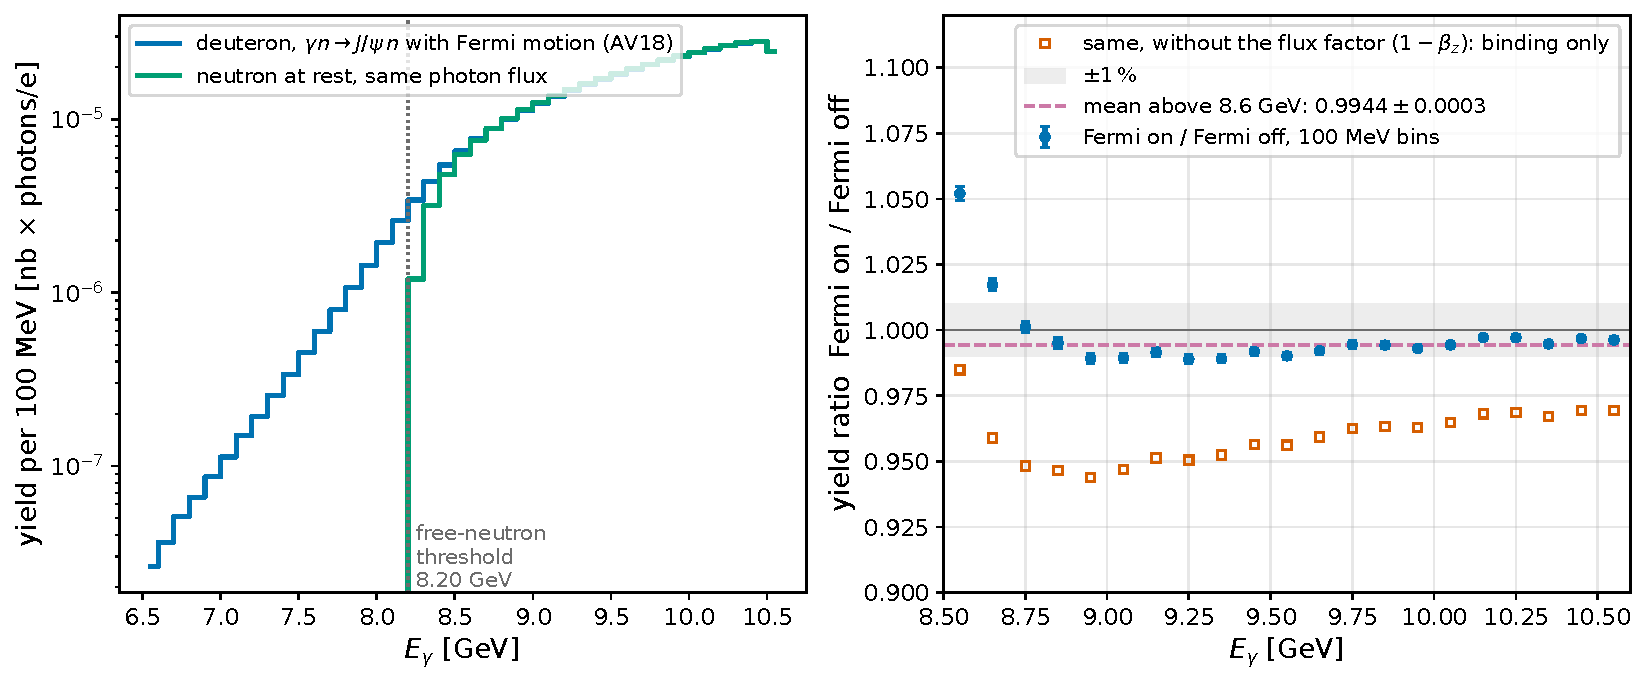
\includegraphics[width=\textwidth]{fig_yield_ratio}
\caption{Left: $\jpsi$ yield per 100\,MeV of photon energy, per incident electron and per neutron,
for the neutron in the deuteron (AV18) and for a free neutron at rest; the free threshold is at
8.20\,GeV.  Right: the ratio of the two above 8.5\,GeV in 100\,MeV bins (filled circles, statistical
errors); the band is $\pm1\,\%$ and the dashed line the mean above 8.6\,GeV.  The open squares show the same ratio when the M\o{}ller
flux factor $1-\beta_{N,z}$ of Eq.~(\ref{eq:weight}) is removed from the deuteron weights: this is
the binding effect alone.}
\label{fig:ratio}
\end{figure}

\begin{table}[htbp]
\centering
\caption{Yield per incident electron and per neutron ($10^{-6}$\,nb$\times$photons/e) in bins of
photon energy, on the deuteron and on the free neutron, their ratio with the statistical error, and
the ratio obtained without the flux factor $1-\beta_{N,z}$ (binding only).}
\label{tab:ratio}
\begin{tabular}{lcccc}
\toprule
$\Eg$ [GeV] & deuteron & free neutron & ratio & ratio without flux factor \\
\midrule
8.2--8.4   & \yOnA & \yOffA & $\ratA\pm\ratErrA$ & \ratNFA \\
8.4--8.6   & \yOnB & \yOffB & $\ratB\pm\ratErrB$ & \ratNFB \\
8.6--9.0   & \yOnC & \yOffC & $\ratC\pm\ratErrC$ & \ratNFC \\
9.0--9.5   & \yOnD & \yOffD & $\ratD\pm\ratErrD$ & \ratNFD \\
9.5--10.0  & \yOnE & \yOffE & $\ratE\pm\ratErrE$ & \ratNFE \\
10.0--10.6 & \yOnF & \yOffF & $\ratF\pm\ratErrF$ & \ratNFF \\
\midrule
6.5--10.6 (all) & \yieldD & \yieldN & \totalRatio & \noFluxTotal \\
\bottomrule
\end{tabular}
\end{table}

Table~\ref{tab:ratio} gives the numbers.  Above 8.6\,GeV the ratio never leaves the band
0.99--1.00: it is $\maxRat\pm\maxErr$ in \maxLo--\maxHi\,GeV, passes through a shallow minimum of
$\minRat\pm\minErr$ in \minLo--\minHi\,GeV, and comes back to $\ratF$ in the last 600\,MeV; its mean
over 8.6--10.6\,GeV is
\begin{equation}
\frac{Y_d}{Y_n}\Big|_{8.6<\Eg<10.6\GeV}=\meanHi\pm\meanHiErr .
\end{equation}
With 20 million events the statistical errors are small enough to resolve this sub-percent shape,
which is why no straight line fits it; what matters is its size.
The total yield per neutron over the whole generated range is $\totalRatio$ times the free-neutron
one; the excess is the near-threshold region, 8.2--8.6\,GeV, and the sub-threshold yield of
Section~\ref{sec:below}.  \textbf{Above 8.6\,GeV Fermi motion does not change the $\jpsi$ yield per
neutron by more than 1\,\%.}  This is the net of two effects that the last column of
Table~\ref{tab:ratio} separates.  Without the flux factor the ratio is $\ratNFE$ at 9.5--10\,GeV: the
struck neutron carries less than its rest energy ($\langle E_N\rangle=M_D-\langle E_s\rangle=0.933\GeV$
against $M_n=0.940\GeV$) and is off shell ($\langle m^*\rangle=\msAb\GeV$), so at fixed $\Eg$ the
average $s$ is lower than on a free neutron by about $0.16\GeV^2$, i.e.\ $W$ by 18\,MeV, and with
$d\ln\sigma/dW\simeq2.7\GeV^{-1}$ the yield drops by 4--5\,\%.  The flux-factor correlation of
Section~\ref{sec:flux} adds back $+4$\,\%.  The two have different energy dependence, both growing
toward threshold, which is why the ratio without the flux factor rises slowly with $\Eg$ from
$\ratNFC$ to $\ratNFF$ while the full ratio stays within 1\,\% of one.

Near the free threshold the picture changes completely.  In 8.4--8.6\,GeV the ratio is $\ratB$, in
8.2--8.4\,GeV it is $\ratA$ (2.6 in the first 100\,MeV above threshold), and below 8.20\,GeV the free-neutron yield is zero while the deuteron
yield is not: Fermi motion smears the sharp threshold of $\sigma_{\rm tot}(W)\propto(W-W_{\rm th})^{0.7}$
over $\pm300$\,MeV of photon energy.  Any extraction of the near-threshold cross section from
deuterium data has to unfold this, and the generator provides the response.

\subsection{The yield below the free threshold}
\label{sec:below}

\begin{figure}[htbp]
\centering
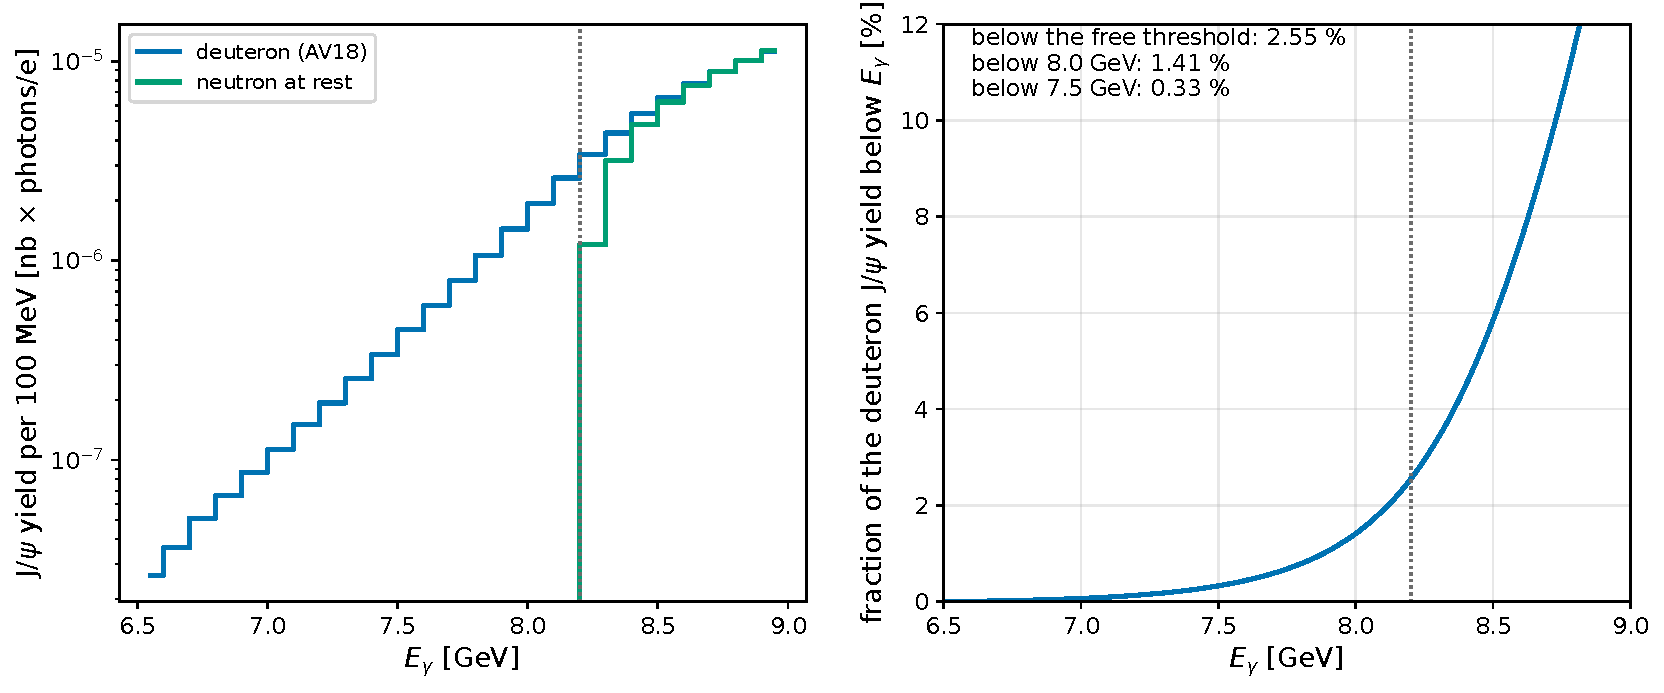
\includegraphics[width=\textwidth]{fig_threshold}
\caption{Left: the yield per 100\,MeV between 6.5 and 9\,GeV on the deuteron and on the free neutron
(logarithmic scale).  Right: cumulative fraction of the deuteron $\jpsi$ yield below a given photon
energy.}
\label{fig:threshold}
\end{figure}

Figure~\ref{fig:threshold} shows the region below and around the free threshold.  On the deuteron
$\fracBelow\,\%$ of the $\jpsi$ yield in the generated range, $\yieldBelow\times10^{-6}$\,nb$\times$
photons per electron, is produced by photons below 8.20\,GeV; $\fracBelowEight\,\%$ below 8.0\,GeV and
$\fracBelowSeven\,\%$ below 7.5\,GeV.  The sample contains \cntA, \cntB, \cntC\ and \cntD\ events in
6.5--7.0, 7.0--7.5, 7.5--8.0 and 8.0--8.2\,GeV.  The yield falls by an order of magnitude per 500\,MeV
below threshold, following the high-momentum tail of $n(\ps)$ folded with the threshold rise of the
cross section, and it depends on exactly the ingredients that are least certain: the AV18 tail beyond
300\,MeV/$c$, the off-shell prescription and the absence of final-state interactions.  The numbers
below 8\,GeV should be read as the plane-wave expectation, good to a factor of order two rather than to
percent.

\subsection{Spectator momenta and the off-shell mass}

\begin{figure}[htbp]
\centering
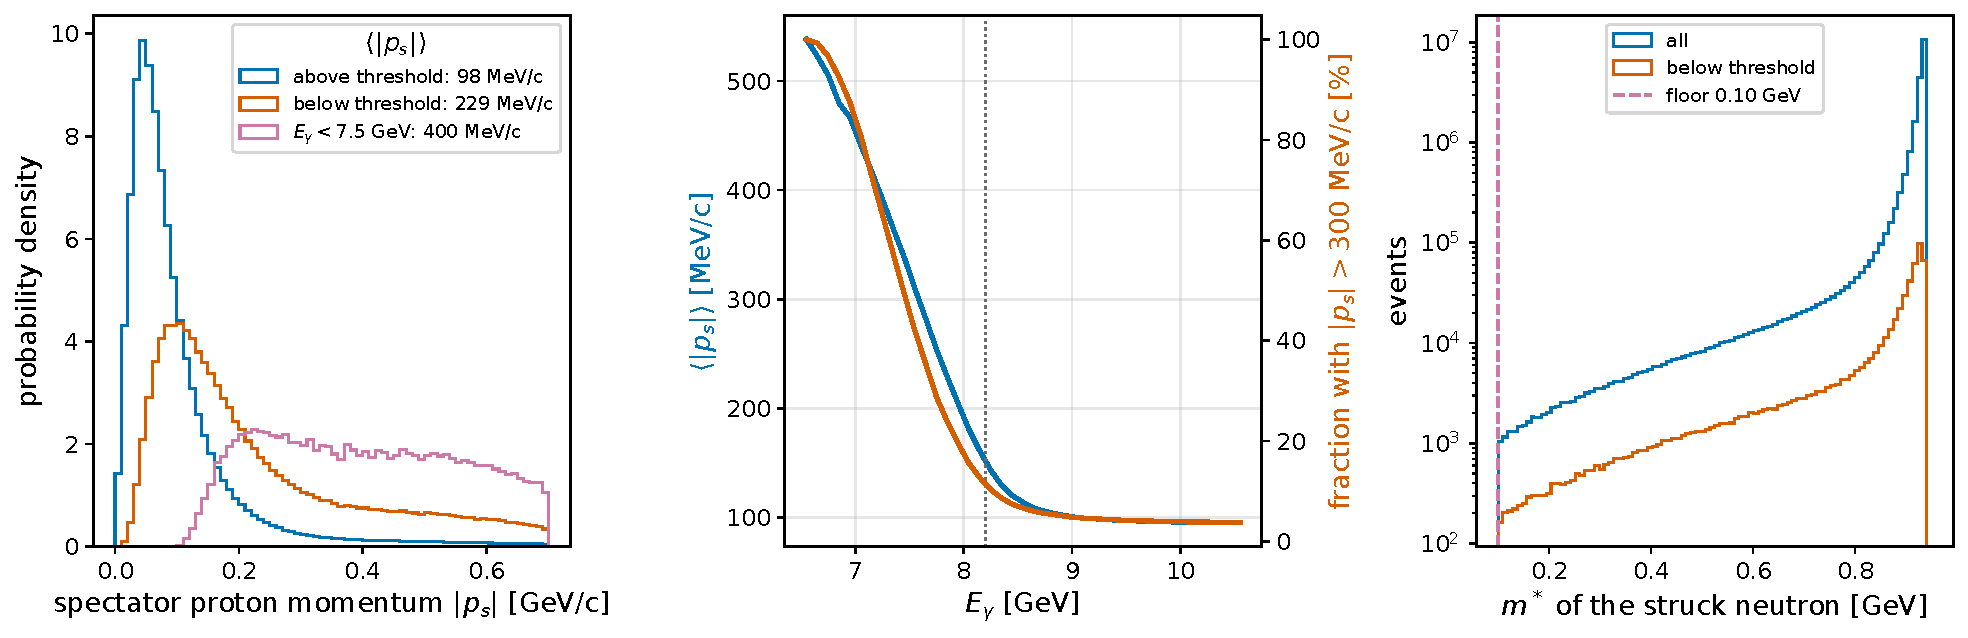
\includegraphics[width=\textwidth]{fig_spectator}
\caption{Left: distribution of the spectator proton momentum for events above the free threshold,
below it, and below 7.5\,GeV.  Middle: mean spectator momentum and the fraction of events with
$\ps>300$\,MeV/$c$ against the photon energy.  Right: the off-shell mass $m^*$ of the struck neutron,
all events and sub-threshold events; the floor at 0.10\,GeV is indicated.}
\label{fig:spectator}
\end{figure}

The spectator proton is written in every deuteron event and Figure~\ref{fig:spectator} shows what it
looks like.  Above the free threshold the spectators follow the bulk of AV18: $\langle\ps\rangle=\psAb$
\,MeV/$c$ and $\fpsAb\,\%$ above 300\,MeV/$c$, with $\langle m^*\rangle=\msAb\GeV$.  Below threshold
the events are selected from the tail: $\langle\ps\rangle=\psBe$\,MeV/$c$ and $\fpsBe\,\%$ above
300\,MeV/$c$ for all sub-threshold events, $\psEi$\,MeV/$c$ and $\fpsEi\,\%$ below 8.0\,GeV,
$\psSe$\,MeV/$c$ and $\fpsSe\,\%$ below 7.5\,GeV, with $\langle m^*\rangle$ falling to $\msSe\GeV$.
The floor at 0.10\,GeV removes 0.01\,\% of the draws overall and is invisible in any of these
distributions.  A sub-threshold $\jpsi$ comes with a fast spectator proton at large angle
that CLAS12 can detect, which is the experimental handle on this part of the sample.

\subsection{The $t$ distributions}

\begin{figure}[htbp]
\centering
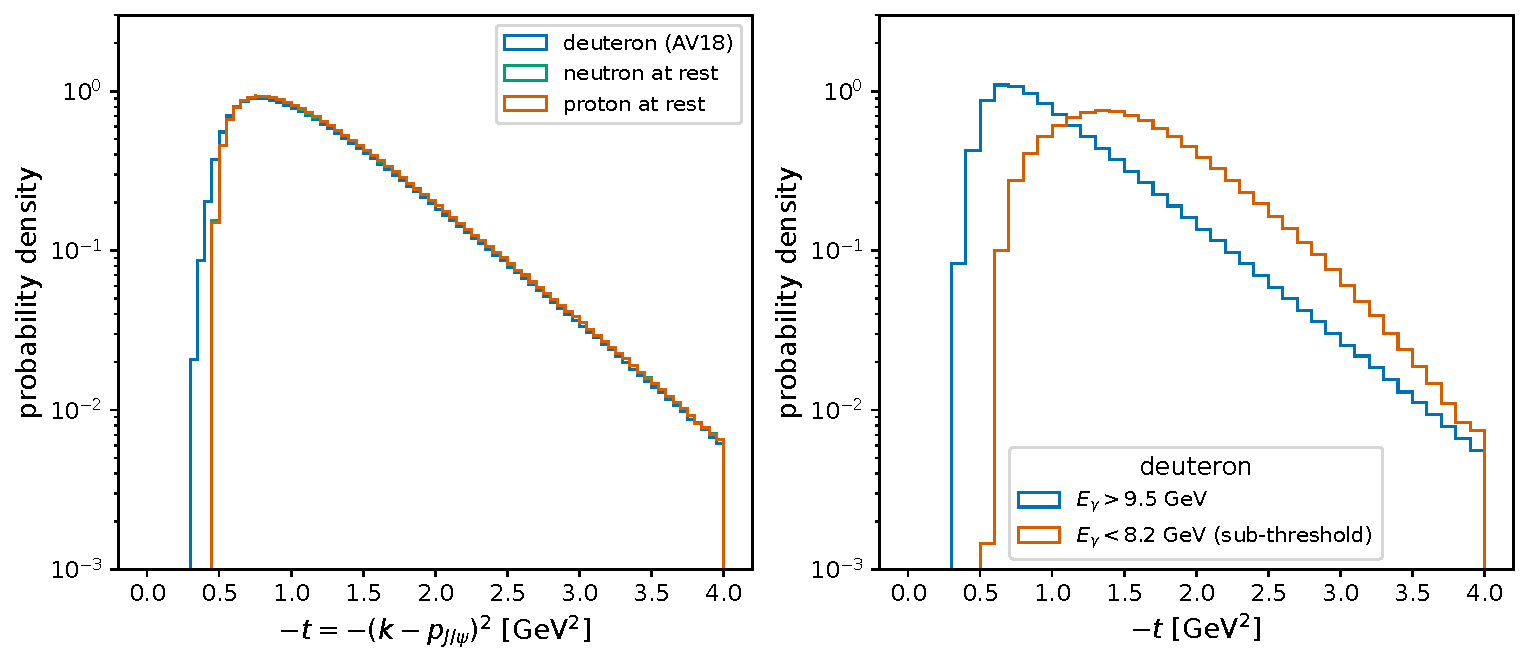
\includegraphics[width=0.95\textwidth]{fig_t}
\caption{Left: $-t=-(k-p_{\jpsi})^2$, with $k$ the photon four-vector, for the three samples.  Right:
on the deuteron, above 9.5\,GeV and below the free threshold.}
\label{fig:t}
\end{figure}

Figure~\ref{fig:t} shows $-t=-(k-p_{\jpsi})^2$, computed as an analysis would from the photon and the
$\jpsi$, without knowledge of the spectator.  Above threshold the deuteron and the free-nucleon
distributions coincide: the $t$ dependence is generated at the event's own $s$ and Fermi motion only
redistributes events among nearby $s$.  Below the free threshold the events sit at the edge of phase
space, $|t|_{\min}$ is large and the distribution is compressed toward it; the $t$ slope of a
sub-threshold sample is not the elementary slope $b$.

\section{Discussion and limits}
\label{sec:discussion}

\paragraph{What the result means.}  For the $\jpsi$ yield per neutron above 8.6\,GeV, a generator
without Fermi motion is as good as one with it, to better than 1\,\% at every photon energy.
This is not because Fermi motion is small (the smearing of $s$ is $\pm0.7\GeV^2$) but because its
two first-order effects on a steeply rising cross section, binding and the flux-factor correlation,
cancel to that level for the AV18 deuteron.  The cancellation is specific to the observable (yield at
fixed lab photon energy, integrated over the spectator) and to the steepness of $\sigma(W)$; it would
not hold for a different $\alpha$ or for a target with larger binding.

\paragraph{Where Fermi motion is essential.}  Within 400\,MeV of the free threshold the ratio departs
from one by tens of percent and below 8.20\,GeV the whole yield is a Fermi-motion effect.  The
$\Eg$-dependence of a threshold measurement on deuterium must be unfolded with this response, and the
spectator proton, when detected, tags the events that carry it.

\subsection{Do we need a Monte Carlo with Fermi motion?}
\label{sec:need}

\begin{figure}[htbp]
\centering
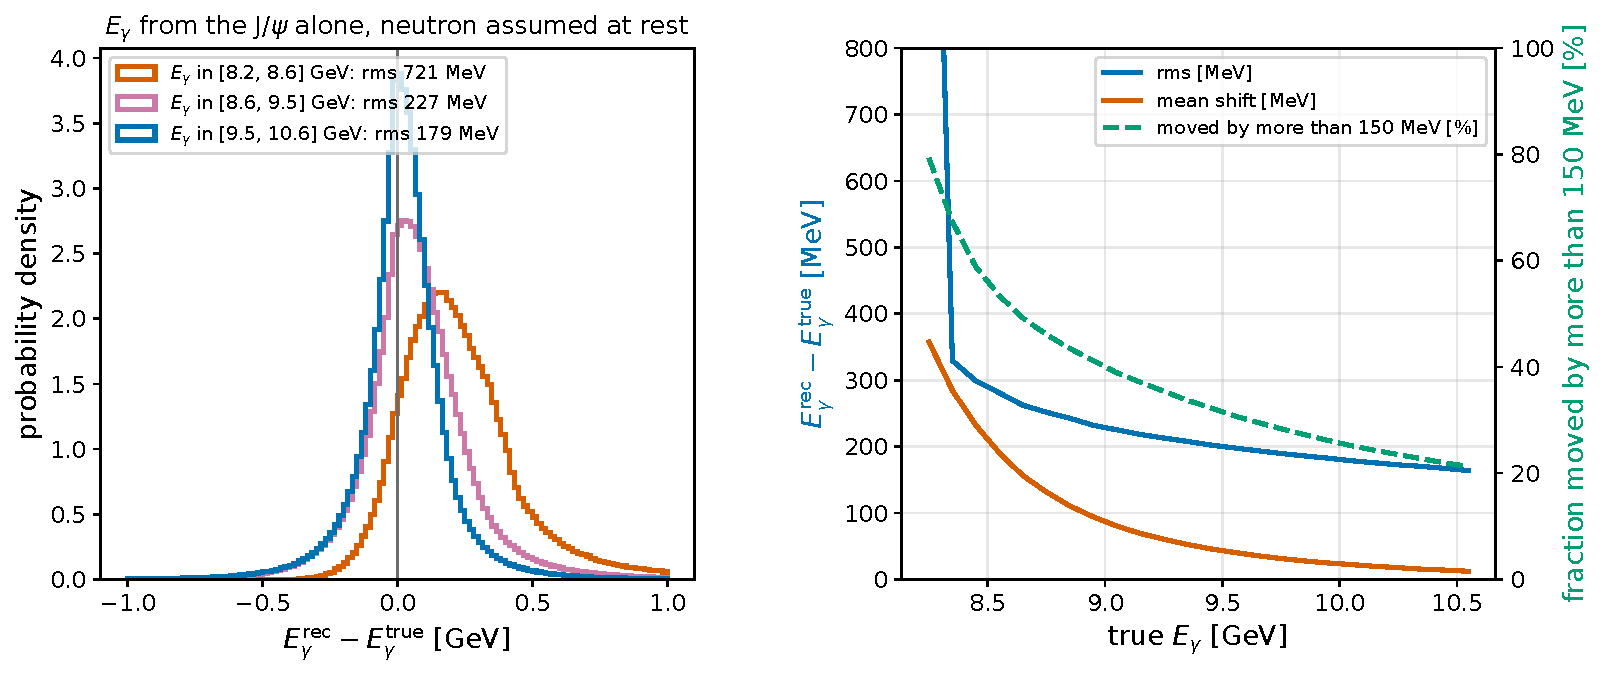
\includegraphics[width=\textwidth]{fig_ereco}
\caption{Photon energy reconstructed from the $\jpsi$ four-vector alone with the target neutron
assumed at rest, as an untagged analysis does it, minus the true photon energy, on the deuteron.
Left: distributions in three ranges of true $\Eg$.  Right: rms and mean shift, and the fraction of
events displaced by more than 150\,MeV, against the true $\Eg$.  On a free neutron all three are zero.}
\label{fig:ereco}
\end{figure}

The answer has two parts, and they point in different directions.

\emph{For the yield per neutron at the true photon energy, no.}  Above 8.6\,GeV a free-neutron
generator reproduces the deuteron yield to better than 1\,\% in every 100\,MeV bin
(Table~\ref{tab:ratio}), and the $t$ distribution at the true $s$ is the same.  If the analysis knew
the photon energy and the momentum transfer event by event, Fermi motion could be switched off.

\emph{For everything an analysis actually measures on deuterium, yes.}  An untagged analysis does
not know $\Eg$; it reconstructs it from the final state with the target at rest, and Fermi motion
enters that reconstruction at full strength.  Figure~\ref{fig:ereco} and Table~\ref{tab:ereco} show
the photon energy obtained from the $\jpsi$ alone, $\Eg^{\rm rec}=(2M_nE_{\jpsi}-M_{\jpsi}^2)/
2(M_n-E_{\jpsi}+p_{z,\jpsi})$: it is smeared by $\erRH$\,MeV rms above 8.6\,GeV, shifted upward by
$\erBB$\,MeV in 8.6--9.0\,GeV and by $\erBA$\,MeV in the bins next to threshold, and
$\erMH\,\%$ of the events move by more than 150\,MeV, i.e.\ out of a typical energy bin.  The
momentum transfer computed with the reconstructed photon is smeared by $\erTH\GeV^2$, comparable to
$1/b$.  A free-neutron Monte Carlo has none of this: it would give the wrong bin migration, the wrong
$t$ resolution, the wrong efficiency of any exclusivity or coplanarity cut, and no events below the
free threshold or with a fast spectator.  The near-threshold region, where the ratio is 1.09 and
1.78 and where the physics interest lies, is entirely a Fermi-motion effect.

Since the deuteron generator costs 0.65\,ms per event and passes every acceptance test, there is
no reason to generate deuterium without it.  The free-neutron sample keeps one role: the cross-check
that isolates the Fermi-motion effect, as in this report.

\begin{table}[htbp]
\centering
\caption{Resolution of the photon energy reconstructed from the $\jpsi$ alone on the deuteron
(neutron assumed at rest): mean shift, rms, fraction of events moved by more than 150\,MeV, and the
rms of the momentum transfer computed with the reconstructed photon minus the true one.}
\label{tab:ereco}
\begin{tabular}{lcccc}
\toprule
true $\Eg$ [GeV] & shift [MeV] & rms [MeV] & moved $>150$\,MeV & $\Delta t$ rms [GeV$^2$] \\
\midrule
8.2--8.6   & \erBA & \erRA & \erMA\,\% & \erTA \\
8.6--9.0   & \erBB & \erRB & \erMB\,\% & \erTB \\
9.0--9.5   & \erBC & \erRC & \erMC\,\% & \erTC \\
9.5--10.0  & \erBD & \erRD & \erMD\,\% & \erTD \\
10.0--10.6 & \erBE & \erRE & \erME\,\% & \erTE \\
\midrule
8.6--10.6  & \erBH & \erRH & \erMH\,\% & \erTH \\
\bottomrule
\end{tabular}
\end{table}

\paragraph{Limits of the model.}  The calculation is plane-wave impulse approximation with a
spectator on shell and the cross section evaluated at the free-nucleon mass.  Not included: final-state
interactions of the $\jpsi$ or the recoil neutron with the spectator, coherent production on the
deuteron, any modification of the elementary amplitude off shell, the $D$-wave tensor structure
(only $|\psi|^2$ enters), and the difference between $\sigma_n$ and $\sigma_p$.  The AV18 tail above
300\,MeV/$c$ is used as is.  The bremsstrahlung is thin-target and does not include the energy loss
before radiation or the beam energy spread, each of order 1\,MeV at the endpoint.  The elementary cross
section is one parametrisation, \texttt{roberts2026}, with $b=1.67\GeV^{-2}$ independent of $W$; the
ratio of Section~\ref{sec:ratio} depends on its slope near threshold, not on its normalisation.

\begin{thebibliography}{9}
\bibitem{clas12jpsi} P.~Chatagnon et al.\ (CLAS Collaboration), \emph{Measurement of the
near-threshold $J/\psi$ photoproduction cross section with the CLAS12 experiment},
arXiv:2602.22128 [hep-ex] (2026), JLAB-PHY-26-4605, submitted to Phys.\ Rev.\ C.
\end{thebibliography}

\appendix

\section{Cards, commands and files}
\label{app:cards}

The deuteron card (\texttt{photo20M/card\_d2.txt}); the neutron and proton cards differ only in the
model (\texttt{jpsin.roberts2026} with \texttt{fermi = none}; \texttt{jpsi.roberts2026}), in
\texttt{target\_X0\_cm = 890.4} for LH$_2$ and in the output directory:
\begin{verbatim}
model = jpsin.roberts2026
ebeam = 10.6
kmin  = 6.5
kmax  = 10.6
tmin  = -6.0
tmax  = -0.001
nev   = 20000000
seed  = 2027
fermi = av18
fermi_mstar_min = 0.10
target_length_cm = 5.0
target_X0_cm = 769.1
vz = -5.5 -0.5
idecay = 1
maj_safety = 1.05
outroot = ROOT/photo20M/d2
\end{verbatim}
Generation, figures and this document:
\begin{verbatim}
python3 -m exclurad_py.generator.photo card_d2.txt --jobs 10
python3 validation/jpsi_photo_report_figs.py ROOT/photo20M ROOT/photo20M/report
python3 validation/numbers_to_tex.py ROOT/photo20M/report/numbers.json numbers.tex
pdflatex jpsi_fermi_photoproduction.tex
\end{verbatim}
The samples (LUND files, 42\,GB) are on the Mac mini, with \texttt{ROOT} the directory
\texttt{/Volumes/wd\_14tb/} \texttt{aao\_norad\_kin/jpsi\_fermi}; each run directory carries its
\texttt{inputs/config.json}.  The figures, \texttt{numbers.json} and this report are in the
\texttt{jpsi-fermi} branch under \texttt{docs/jpsi\_fermi/report/}, and in the OneDrive folder
\texttt{Work/2026\_Jpsi\_Fermi\_photoproduction}.

\end{document}
